We now discuss how different predictions compare when the matching to parton shower is included. For such
a comparison we expect larger discrepancy than what we found at fixed-order, as a consequence of the different
matching schemes, parton shower employed, and of other details of the matching (such as the choice of the parton shower initial scale). Among
the codes capable of providing fixed-order results, presented before, {\sc MG5\_aMC}, the {\sc Powheg-Box}, and {\sc VBFNLO}
can also provide results at (N)LO+PS accuracy. For {\sc VBFNLO} matched to {\sc Herwig} and the {\sc Powheg-Box}, we
restrict ourselves to showing results only in the VBS approximation,
{\emph i.e.}\ the $s$-channel contributions are neglected here. Besides,
also {\sc PHANTOM} is used for LO+PS results.\\
{\sc MG5\_aMC}, which
employs the {\sc MC@NLO}~\cite{Frixione:2002ik} matching procedure, will be used together with {\sc Pythia8}~\cite{Sjostrand:2014zea} (version 8.223)
and {\sc Herwig++}~\cite{Bahr:2008pv, Bellm:2013hwb} (version 2.7.1). The same parton showers will be employed for the LO results of {\sc PHANTOM}. For the {\sc Powheg-Box}, the namesake
matching procedure is employed~\cite{Nason:2004rx,Frixione:2007vw}, together with {\sc Pythia8} (version 8.230). {\sc VBFNLO} serves as a matrix-element and phase-space provider
for the {\sc Matchbox} module~\cite{Platzer:2011bc} of {\sc
Herwig7}~\cite{Bellm:2015jjp,Bellm:2017bvx}, using an extended version of the BLHA
interface~\cite{Binoth:2010xt,Alioli:2013nda,Andersen:2014efa}. The {\sc Matchbox} module makes it
possible to choose between {\sc MC\-@NLO}-like and {\sc Powheg}-like
matching. As parton shower, both the default angular-ordered shower as
well as the dipole shower can be employed.
Whenever {\sc Pythia8}\ is used, the Monash tune~\cite{Skands:2014pea} is selected.

Results will be presented within the cuts described in Sec.~\ref{subsec:inputpar}, applied after shower and hadronisation (this implies that jets
are obtained by clustering stable hadrons, and not QCD partons). It follows that at the event-generation level, looser cuts (or even no cuts at all)
must be employed in order not to bias the results. 

Compared to the fixed order computations, a slightly different set-up has been employed for {\sc MG5\_aMC} in order to simplify the calculation: instead of generating the full
${\rm p}{\rm p}\to\mu^+\nu_\mu{\rm e}^+\nu_{\rm e}{\rm j}{\rm j}$ process, since it is dominated by doubly-resonant contribution, the
events are produced for the process with two stable ${\rm W}^+$-bosons (${\rm p}{\rm p}\to{\rm W^+}{\rm W^+}{\rm j}{\rm j}$), and the decay of these ${\rm W}^+$-bosons
is simulated with {\sc MadSpin}~\cite{Artoisenet:2012st} (ensuring spin correlations) before the PS. Since {\sc MadSpin}\ computes
the partial and total decay width of the W bosons at LO accuracy only, while in Section~\ref{subsec:inputpar} the NLO width is employed,
an effect ($6\%$) on the normalisation is induced. Finally, when the renormalisation
and factorisation scales are set, the $\Delta R_{\Pj\Pl}$ cut is not imposed during the jet-clustering procedure.
This effect is below a per cent at the level of the fiducial cross sections.

\begin{table}[h!]
    \centering
    \begin{tabular}{c|l@{ $\pm$ }l}
      Code  &  \multicolumn{2}{c}{$\sigma[\rm{fb}]$}  \\
        \hline\hline
        {\sc MG5\_aMC}+{\sc Pythia8}&  $1.352 $ & $0.003$  \\
        {\sc MG5\_aMC}+{\sc Herwig++}&  $1.343 $ & $ 0.003$  \\
        {\sc MG5\_aMC}+{\sc Pythia8}, $\Gamma_{\rm resc}$&  $1.275$ & $0.003$  \\
        {\sc MG5\_aMC}+{\sc Herwig++}, $\Gamma_{\rm resc}$&  $1.267$ & $ 0.003$  \\
        {\sc PHANTOM}+{\sc Pythia8} &  $1.235 $ & $0.001$  \\
        {\sc PHANTOM}+{\sc Herwig++} &  $1.260 $ & $0.001$  \\
        {\sc VBFNLO}+{\sc Herwig7-Dipole} &  $1.3001$ & $0.0002$  \\
    \end{tabular}
    \caption{\label{tab:PSratesLO} Cross sections at LO+PS accuracy.
    The {\sc MG5\_aMC} results with $\Gamma_{\rm resc}$ 
    are rescaled to account for the effect related to the boson widths computed by {\sc MadSpin} (see the text for details).
    The uncertainties shown refers to estimated statistical error of the Monte Carlo programs.}
\end{table}

\begin{table}[h!]
    \centering
    \begin{tabular}{c|l@{ $\pm$ }l}
      Code  &  \multicolumn{2}{c}{$\sigma[\rm{fb}]$}  \\
        \hline\hline
        {\sc MG5\_aMC}+{\sc Pythia8}&  $1.450 ^{+2\%}_{-1\%} {}^{+2\%}_{-2\%} $ & $0.004$  \\
        {\sc MG5\_aMC}+{\sc Herwig++}&  $1.445 $ & $0.004$  \\
        {\sc MG5\_aMC}+{\sc Pythia8}, $\Gamma_{\rm resc}$&  $1.368$ & $0.004$  \\
        {\sc MG5\_aMC}+{\sc Herwig++}, $\Gamma_{\rm resc}$&  $1.363$ & $0.004$  \\
        {\sc Powheg-Box}  & $1.3642$ & $0.0004$  \\
        {\sc VBFNLO}+{\sc Herwig7-Dipole} &  $1.3389 ^{+0\%}_{-1\%}$ & $0.0006$  \\
        {\sc VBFNLO}+{\sc Herwig7-Default} &  $1.3067$ & $0.0006$  \\
    \end{tabular}
    \caption{\label{tab:PSratesNLO} Cross sections at NLO+PS accuracy.
    The {\sc MG5\_aMC} results with $\Gamma_{\rm resc}$ 
    are rescaled to account for the effect related to the boson widths computed by {\sc MadSpin} (see the text for details). For
    {\sc VBFNLO}+{\sc Herwig7-Dipole}, the three-point scale uncertainties are shown, while for  {\sc MG5\_aMC}+{\sc Pythia8} the two displayed uncertainties
are respectively the nine-point scale uncertainty and the PDF one.
The uncertainties shown refers to estimated statistical error of the Monte Carlo programs.}
\end{table}

We now present the results of predictions matched to parton shower.
The total rates within VBS cuts are displayed in Tables~\ref{tab:PSratesLO} and
\ref{tab:PSratesNLO}, at LO and NLO
accuracy respectively. For {\sc MG5\_aMC}, 
the numbers with $\Gamma_{\rm resc}$ are rescaled to 
take into account the width effects described in the above paragraph. At NLO accuracy, for {\sc MG5\_aMC} + {\sc Pythia8} and {\sc VBFNLO}-{\sc Dipole}, we also quote
theoretical uncertainties.
For the former, we show both PDF and scale uncertainties,\footnote{A preliminary study on PDF uncertainties in VBS has appeared 
in Ref.~\cite{Schwan:2017yy}.} obtained via exact reweighting~\cite{Frederix:2011ss} by varying independently the renormalisation and factorization
scale by a factor of two around its central value, Eq.~(\ref{eq:defscale}) (nine-point variations).
For the latter, we show the 
three-point scale uncertainties, obtained by considering correlated variations of the renormalisation and factorisation scales. Theory uncertainties should have very little dependence on the tool employed.
We observe that, once the width effect is taken into
account, total rates from different tools agree within a few per cent, both at LO and NLO. Larger discrepancies, however, will appear for differential observables, which we are going to discuss in
the following. Before turning to the differential observables, we point out the smallness of the theory uncertainties due to the scale variations, both when
scales are varied independently and when they are varied in a correlated manner, as well as those due to PDF.  
Concerning differential distributions, for each observable we will display results in two plots, shown side-by-side. In the plot on the left (right), (N)LO+PS predictions are shown
with different colours in the main frame. In the inset, these predictions are compared in both cases with a fixed-order prediction at NLO accuracy (obtained with
{\sc VBFNLO}, \emph{i.e.}\ the VBS approximation with $s$-channel).
For the differential observables, the {\sc MG5\_aMC} predictions are \emph{not} rescaled to compensate for the width effect mentioned above. As for the table, we show theoretical uncertainties for the NLO+PS samples
obtained with {\sc VBFNLO} and {\sc MG5\_aMC}: 
again, for the first the band corresponds to three-point variations, while for the second the darker (lighter) band corresponds to nine-point 
scale variations (plus PDF uncertainties, linearly added). 

The first observable we investigate is the exclusive jet multiplicity, shown in Fig.~\ref{fig:PSnjet}. Looking at the LO+PS predictions, one can appreciate that the
main effects are driven by the parton shower that is employed ({\sc Herwig++/7} or {\sc Pythia8}), with the clear tendency of producing more radiation for the latter,
leading to higher jet multiplicities. Difference among tools that employ the same parton shower are typically smaller, and can be traced back to different values of the
initial scale of the parton shower (the {\tt scalup} entry of the LHE file). This event-by-event number corresponds 
to the maximum hardness (translated into the shower evolution variable) of the radiation that 
can be generated by the shower. \footnote{At LO, the choice of such a scale is arbitrary and usually driven by common sense, 
as it is the case for the factorisation and renormalisation scales.
    At NLO, one has the freedom to change the shower scale without losing formal NLO accuracy within the {\sc MC@NLO} matching, 
    provided the Monte Carlo counterterms are also consistently
updated. In the {\sc Powheg} matching, the shower scale of the so-called $\tilde B$ events is fixed to the transverse momentum of the radiation 
generated according the {\sc Powheg} Sudakov factor, while it can be changed in the remnants events.}
The main effect of NLO corrections for this (rather inclusive) observable is to stabilise the predictions for the two-jet bin, where discrepancies
among tools are reduced to about $10\%$. For the three-jet bin, which is described only at LO accuracy, differences among tools remain large: the largest rate is predicted by
{\sc MG5\_aMC}, while the smallest rate is predicted by the {\sc Powheg-Box}, both matched to {\sc Pythia8}. Despite the fact that the same parton shower is employed, the way emissions are treated
is different among the two tools. In particular, for the {\sc Powheg-Box}, the first emission is generated with an internal Sudakov form factor (the
prediction dubbed {\sc Powheg-no shower} corresponds to stopping after the first emission), while for {\sc MG5\_aMC} there is an
interplay between the real-emission matrix element and the shower emission.

\begin{figure*}[hbt]
\centering
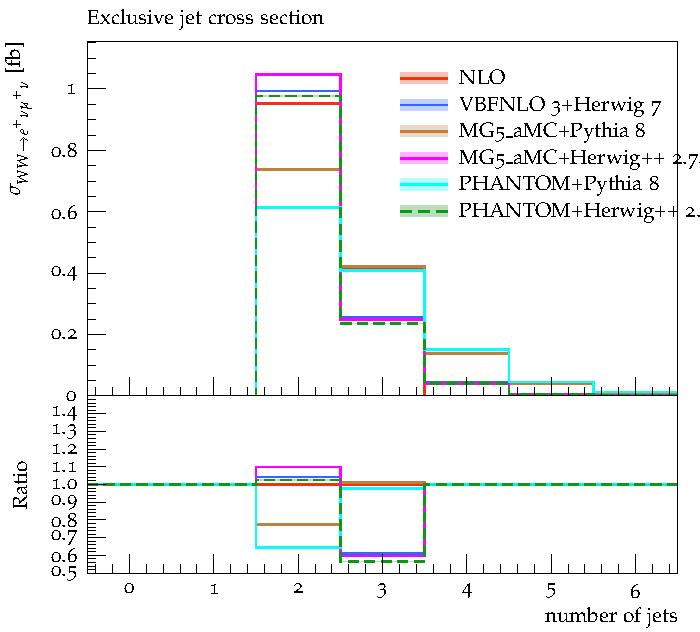
\includegraphics[width=0.47\textwidth]{figures/LOPS/jetsexclusive.pdf}
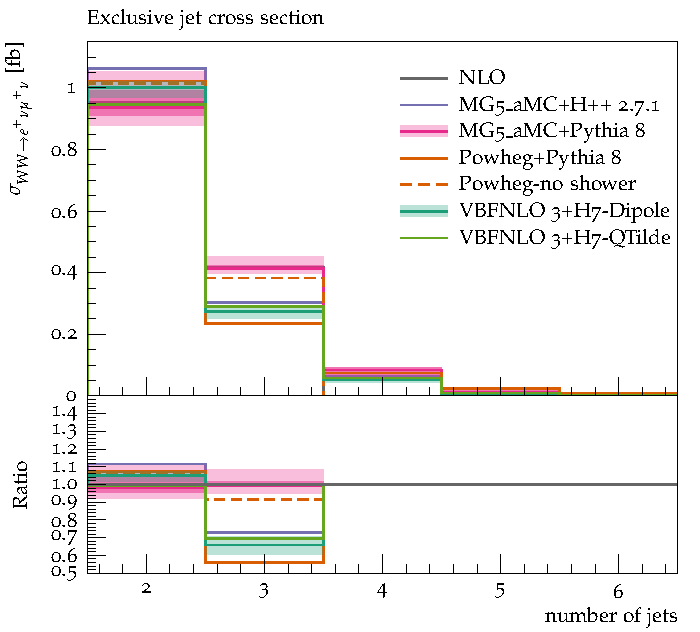
\includegraphics[width=0.47\textwidth]{figures/NLOPS/jetsexclusive.pdf}
\caption{Differential distribution in the 
exclusive jet multiplicity
from predictions matched to parton shower, at LO (left) or NLO (right) accuracy (upper plot), compared with the fixed-NLO result computed with {\sc VBFNLO} (lower plot). At NLO+PS accuracy, for
    {\sc VBFNLO}+{\sc Herwig7-Dipole}, the three-point scale uncertainties are shown, while for {\sc MG5\_aMC}+{\sc Pythia8} the darker and lighter bands correspond  
    respectively to the nine-point scale uncertainty and the scale and PDF uncertainties combined linearly. 
    The predictions are obtained in the fiducial region described in Sec.~\ref{subsec:inputpar}.}
\label{fig:PSnjet}
\end{figure*}
 
\begin{figure*}[hbt]
\centering
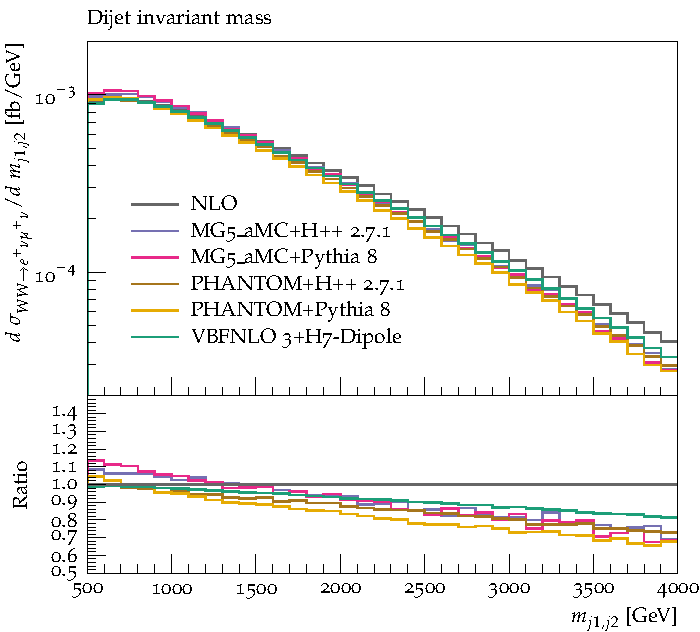
\includegraphics[width=0.47\textwidth]{figures/LOPS/m_jj.pdf}
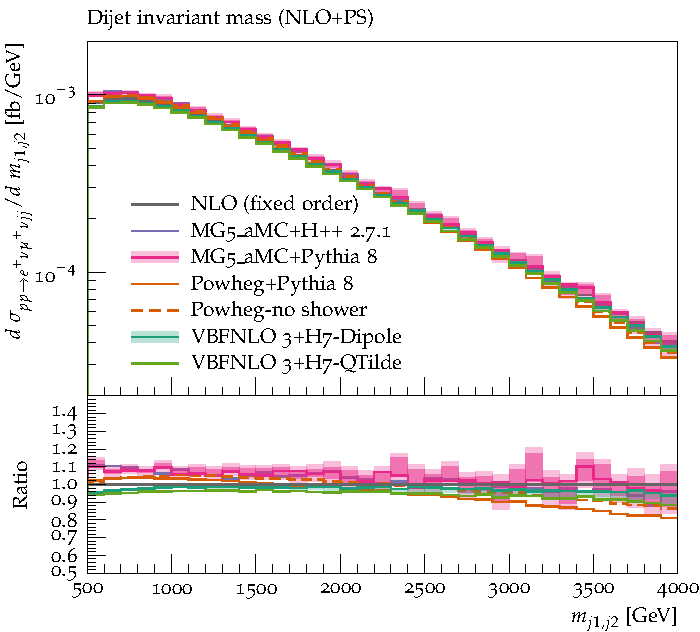
\includegraphics[width=0.47\textwidth]{figures/NLOPS/m_jj.pdf}
\caption{Differential distribution in the 
invariant mass of the two tagging jets
from predictions matched to parton shower, at LO (left) or NLO (right) accuracy (upper plot), compared with the fixed-NLO result computed with {\sc VBFNLO} (lower plot). At NLO+PS accuracy, for
    {\sc VBFNLO}+{\sc Herwig7-Dipole}, the three-point scale uncertainties are shown, while for {\sc MG5\_aMC}+{\sc Pythia8} the darker and lighter bands correspond  
    respectively to the nine-point scale uncertainty and the scale and PDF uncertainties combined linearly. 
    The predictions are obtained in the fiducial region described in Sec.~\ref{subsec:inputpar}.}
\label{fig:PSmjj}
\end{figure*}

The next observable that we study is the invariant mass of the two tagging jets, shown in Fig.~\ref{fig:PSmjj}. For this observable, both at LO+PS and NLO+PS,
the spread of predictions matched with parton shower is rather small
($\lesssim 10\%$, if one compensates for the $6\%$ width effect for {\sc MG5\_aMC}).
The LO+PS predictions tend to be significantly softer than the fixed NLO one, with an effect of
about -30\% at the end of the displayed range. At NLO+PS, this effect is much more mitigated, owing to the better description of the first QCD emission which is now driven by the real-emission matrix element.
 
The rapidity difference between the two tagging jets, shown in Fig.~\ref{fig:PSdyjj}, has some similarities to the invariant-mass distribution.
At LO+PS all predictions,
except for {\sc VBFNLO+Herwig7} where the effect is mitigated, show the tendency to deplete the large-separation region with respect to the fixed-order prediction, in a
quantitatively similar way. At NLO+PS, when the extra radiation is described by the real matrix element, such an effect is greatly reduced. A notable
exception is the {\sc Powheg-Box} prediction, which still shows a suppression at large separations.
Since such a suppression is already there for the {\sc Powheg-no shower} sample,
it is very likely that it is driven by the way the first emission is generated. A minor effect in the same direction is visible in the last two bins of the
{\sc MG5\_aMC+Herwig++} prediction (although with rather large statistical uncertainties).



The transverse momentum of the hardest and second-hardest jets are shown in Figs.~\ref{fig:PSpt1} and~\ref{fig:PSpt2}, respectively. In general, for both observables,
predictions from different tools agree rather well with each other, with a spread at most at the 10\% level. At LO+PS, typically the transverse-momentum spectra are softer than
the fixed-NLO ones, and this effect is more marked for the second-hardest jet which, as expected, is more sensitive to the description of the extra radiation. Again, this
effect is mitigated by NLO corrections. The only feature that may be worth noticing among the NLO+PS predictions is the tendency of the {\sc Powheg-Box} to suppress the
hardest-jet spectrum at low transverse momentum ($\ptsub{\Pj_1}<100 \GeV$).\\
If we consider the rapidity of the second jet, Fig.~\ref{fig:PSy2}, we observe again rather small differences among tools, with the tendency towards a general
stabilisation at NLO+PS. However, some (small) differences in the shape remain at NLO+PS, which are worth to be briefly discussed: predictions
obtained with {\sc MG5\_aMC} are very close to the fixed-order prediction; the {\sc Powheg-Box}\ displays an enhancement of the central region, and a consequent suppression in the
peripheral region, while {\sc VBFNLO} shows an opposite behaviour. However, the effect is rather small, with the largest departure from the fixed-order prediction being
at most $10\%$.\footnote{If the setting {\tt SpaceShower:dipole\-Recoil = on} (discussed in the following) 
is used when {\sc Pythia8}\ is employed together with the {\sc Powheg-Box}, the enhancement at central rapidities and the depletion 
at small value of transverse momentum are partially compensated.}

Finally, focusing on the third jet, we conclude the list of differential observables by showing the Zeppenfeld variable defined in Eq.~\eqref{eq:Zeppenfeld}, Fig.~\ref{fig:PSz3}. This 
variable is closely related to the third jet rapidity, and small (large) values of $z$ correspond to central (peripheral) rapidities. In general, for observables which involve the third jet, one
can clearly see a degradation of the agreement among the various tools, because of the poorer perturbative description of these observables. The Zeppenfeld variable is 
a striking example: both at LO and NLO, the tendency of {\sc Pythia8} to generate more hard and central radiation, corresponding to low values of $z$,
is clearly visible. Such an effect, which is related to the way {\sc Pythia8} deals with the recoil of the radiation in VBF(VBS)-type processes,
can be mitigated by setting {\tt SpaceShower:dipole\-Recoil = on} in the {\sc Pythia8} input file.\footnote{This requires version $\ge8.230$. 
Note that such a setting is not compatible with the NLO matching
in {\sc MG5\_aMC} (but it is compatible with the {\sc Powheg} matching). Also, this setting has other 
effects, though smaller, on the rapidity spectra of the two hardest jets.} It is interesting to notice that
the effect survives beyond the first emission, as it can be observed by comparing {\sc Powheg-no shower} with {\sc Powheg+ Pythia8}. A similar
behaviour of {\sc Pythia8}
has also been observed in the study of EW production of a $\PZ$ boson in association with two jets (see the recent CMS measurement, 
Ref.~\cite{Sirunyan:2017jej} Figure 12), where the experimental data seem to prefer the description by {\sc Herwig++}. 
The central enhancement
is a bit mitigated if NLO+PS tools are used (compare LO+PS and NLO+PS from {\sc MG5\_aMC+Pythia8} with the fixed-NLO prediction), however even at NLO+PS the central region
($z_{j_3}<0.5$) is cursed by huge differences between tools. Large differences, reaching a factor 2, persist also away from the central region. \\

In conclusion, the comparison of tools including matching to parton shower clearly shows the benefits of the inclusion of NLO corrections: for most observables described
effectively at NLO accuracy differences between tools are at (or below) the $10\%$ level. 
Some exceptions exist, \emph{e.g.}\ the rapidity separation of the two tagging jets, which
on the one hand clearly suggest not to rely on a single tool/parton shower, and on the other make it worth to investigate more in details the way QCD radiation is
generated, \emph{e.g.}\ when fully-differential computations at NNLO will become available (for VBF Higgs production, see Refs.~\cite{Cacciari:2015jma, Cruz-Martinez:2018rod}). It is a remarkable fact that, even for those observables that display small discrepancies,
the theoretical uncertainty obtained via scale variations systematically underestimates the spread of predictions. Again, this stresses the need
 to employ at least two different tools in order to obtain a conservative estimate of theoretical uncertainties. Finally, the size of discrepancies for observables that are described at a lower perturbative accuracy, notably those related to the third jet, suggest that
experimental analyses should rely as little as possible on those observables and, in any case, use conservative estimate of the theory 
uncertainties. On the one hand, in order to improve the
description of these observables, a simulation of VBS+j at NLO accuracy, currently unavailable but within the reach of modern 
automated tools, is certainly desirable.
On the other hand, measurements of processes with similar 
color flow (EW production of a single vector boson plus jets,
VBF, \ldots) can certainly help in order to discriminate which tools perform better in the comparison with data~\cite{Aaboud:2017emo,Sirunyan:2017jej}.

\begin{figure*}[hbt]
\centering
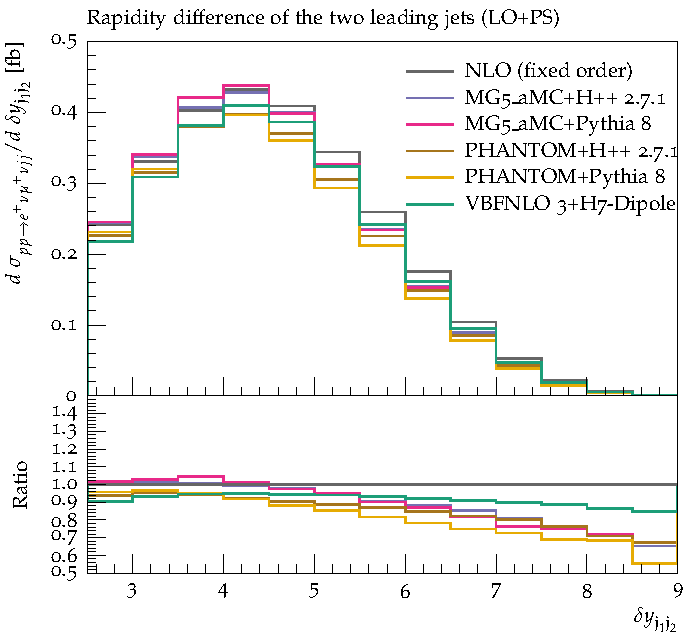
\includegraphics[width=0.47\textwidth]{figures/LOPS/Deltay_jj.pdf}
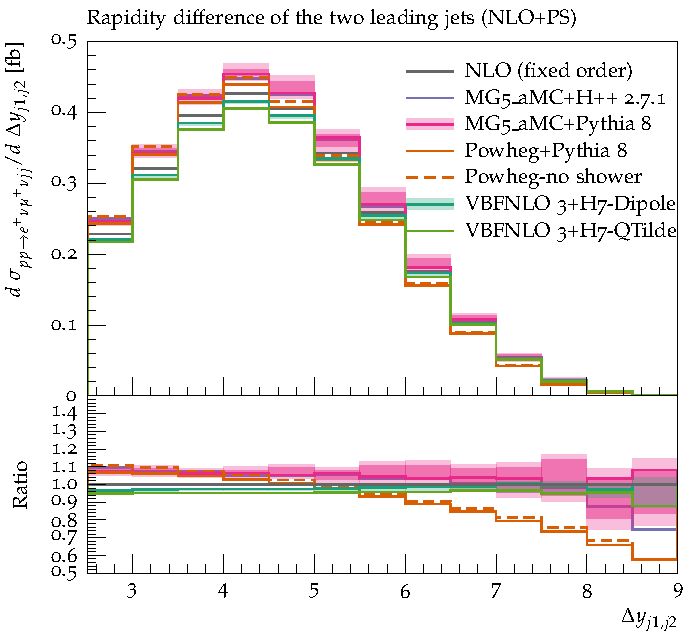
\includegraphics[width=0.47\textwidth]{figures/NLOPS/Deltay_jj.pdf}
\caption{Differential distribution in the 
rapidity separation of the two tagging jets
from predictions matched to parton shower, at LO (left) or NLO (right) accuracy (upper plot), compared with the fixed-NLO result computed with {\sc VBFNLO} (lower plot). At NLO+PS accuracy, for
    {\sc VBFNLO}+{\sc Herwig7-Dipole}, the three-point scale uncertainties are shown, while for {\sc MG5\_aMC}+{\sc Pythia8} the darker and lighter bands correspond  
    respectively to the nine-point scale uncertainty and the scale and PDF uncertainties combined linearly. 
    The predictions are obtained in the fiducial region described in Sec.~\ref{subsec:inputpar}.}
\label{fig:PSdyjj}
\end{figure*}

\begin{figure*}[hbt]
\centering
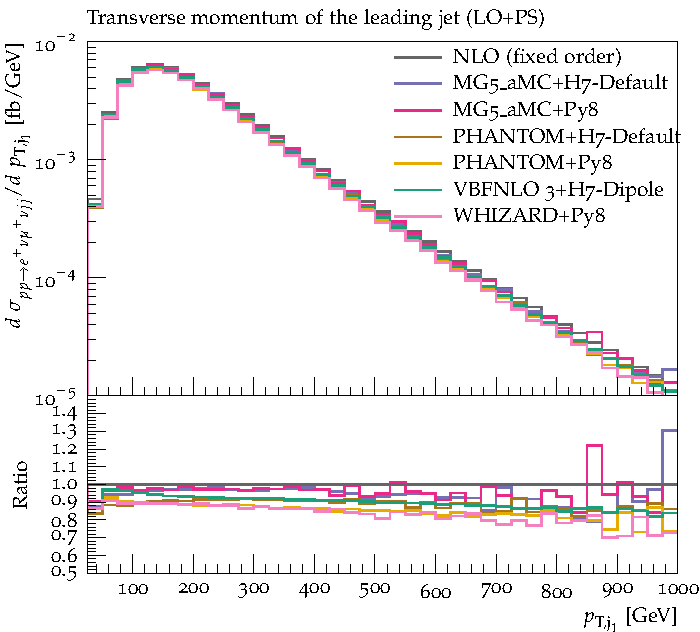
\includegraphics[width=0.47\textwidth]{figures/LOPS/pT_j1.pdf}
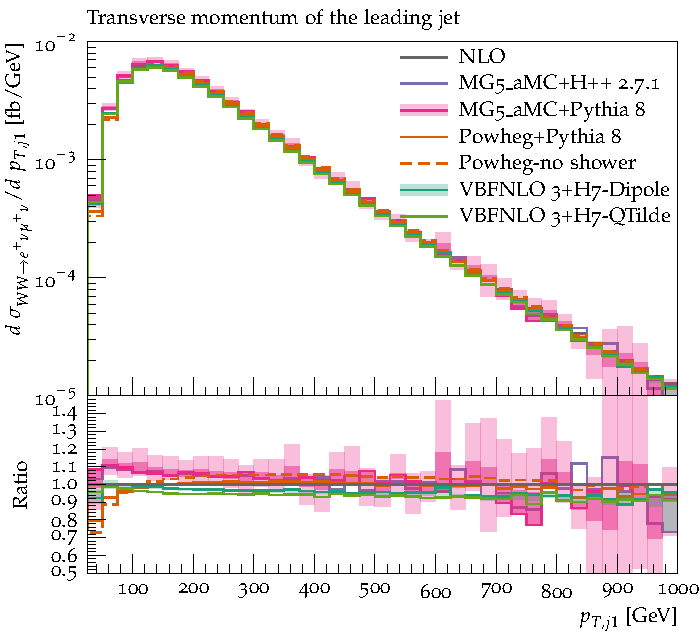
\includegraphics[width=0.47\textwidth]{figures/NLOPS/pT_j1.pdf}
\caption{Differential distribution in the 
transverse momentum of the hardest jet
from predictions matched to parton shower, at LO (left) or NLO (right) accuracy (upper plot), compared with the fixed-NLO result computed with {\sc VBFNLO} (lower plot). At NLO+PS accuracy, for
    {\sc VBFNLO}+{\sc Herwig7-Dipole}, the three-point scale uncertainties are shown, while for {\sc MG5\_aMC}+{\sc Pythia8} the darker and lighter bands correspond  
    respectively to the nine-point scale uncertainty and the scale and PDF uncertainties combined linearly. 
    The predictions are obtained in the fiducial region described in Sec.~\ref{subsec:inputpar}.}
\label{fig:PSpt1}
\end{figure*}

\begin{figure*}[hbt]
\centering
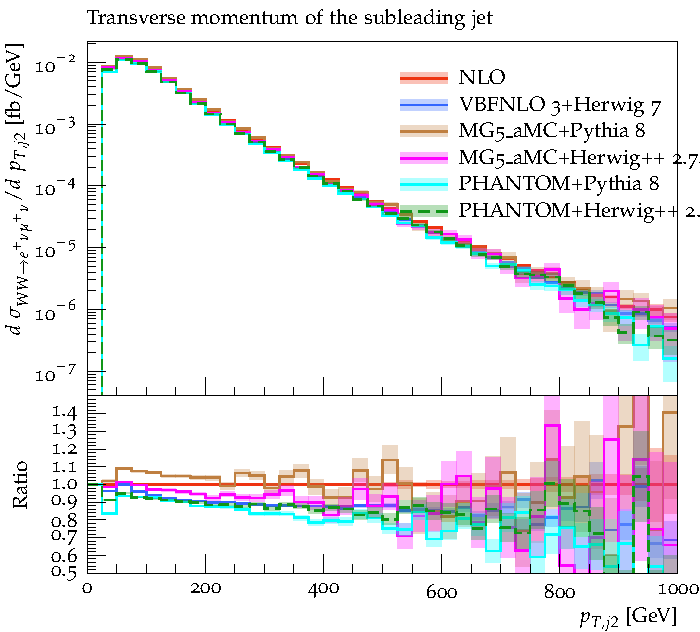
\includegraphics[width=0.47\textwidth]{figures/LOPS/pT_j2.pdf}
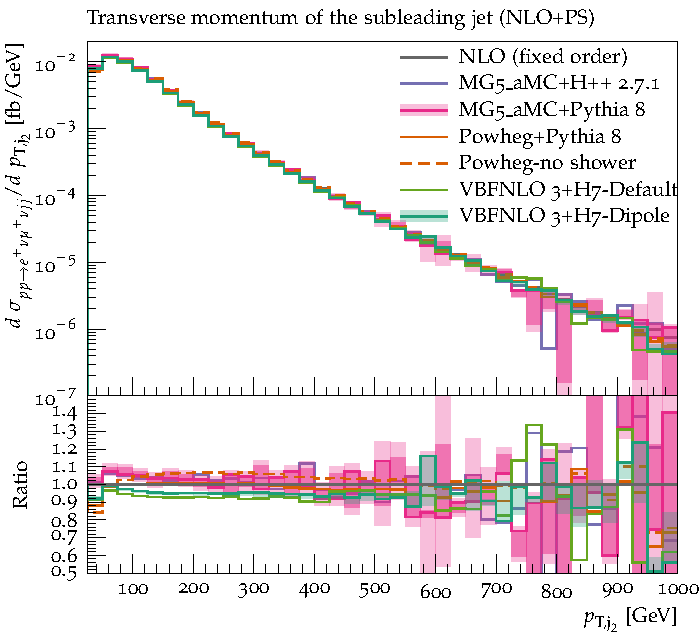
\includegraphics[width=0.47\textwidth]{figures/NLOPS/pT_j2.pdf}
\caption{Differential distribution in the 
transverse momentum of the second-hardest jet
from predictions matched to parton shower, at LO (left) or NLO (right) accuracy (upper plot), compared with the fixed-NLO result computed with {\sc VBFNLO} (lower plot). At NLO+PS accuracy, for
    {\sc VBFNLO}+{\sc Herwig7-Dipole}, the three-point scale uncertainties are shown, while for {\sc MG5\_aMC}+{\sc Pythia8} the darker and lighter bands correspond  
    respectively to the nine-point scale uncertainty and the scale and PDF uncertainties combined linearly. 
    The predictions are obtained in the fiducial region described in Sec.~\ref{subsec:inputpar}.}
\label{fig:PSpt2}
\end{figure*}

\begin{figure*}[hbt]
\centering
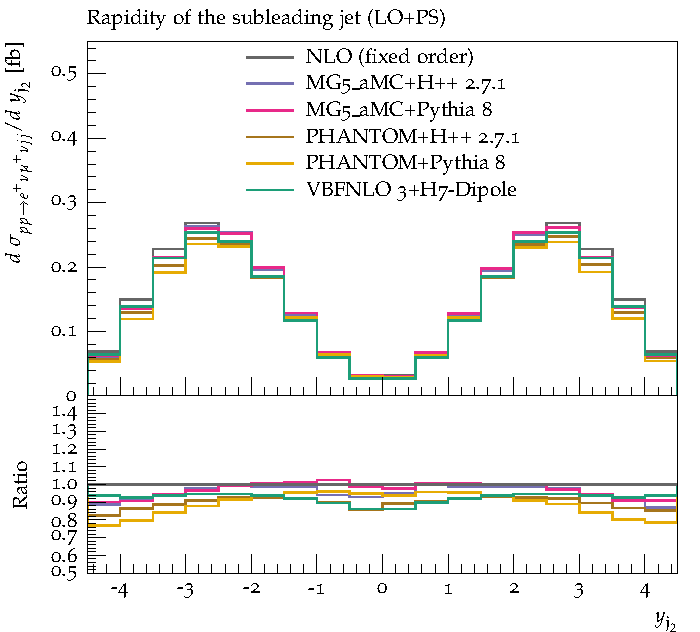
\includegraphics[width=0.47\textwidth]{figures/LOPS/y_j2.pdf}
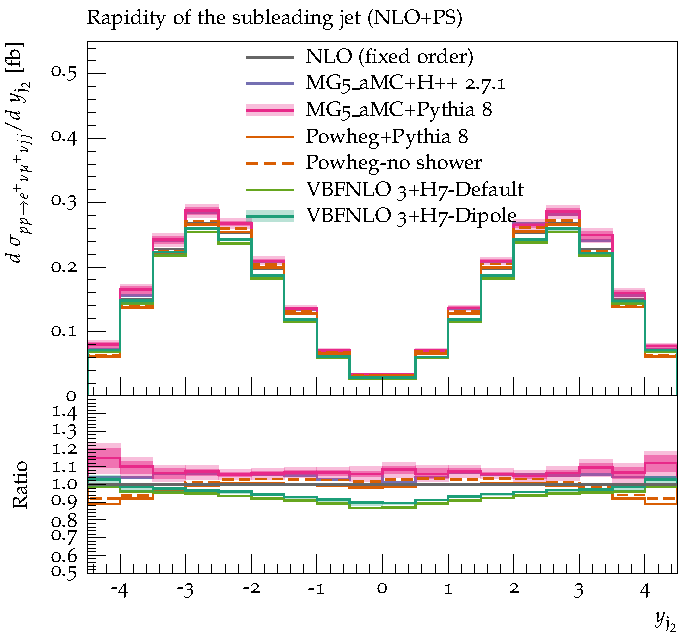
\includegraphics[width=0.47\textwidth]{figures/NLOPS/y_j2.pdf}
\caption{Differential distribution in the 
rapidity of the second-hardest jet
from predictions matched to parton shower, at LO (left) or NLO (right) accuracy (upper plot), compared with the fixed-NLO result computed with {\sc VBFNLO} (lower plot). At NLO+PS accuracy, for
    {\sc VBFNLO}+{\sc Herwig7-Dipole}, the three-point scale uncertainties are shown, while for {\sc MG5\_aMC}+{\sc Pythia8} the darker and lighter bands correspond  
    respectively to the nine-point scale uncertainty and the scale and PDF uncertainties combined linearly. 
    The predictions are obtained in the fiducial region described in Sec.~\ref{subsec:inputpar}.}
\label{fig:PSy2}
\end{figure*}

\begin{figure*}[hbt]
\centering
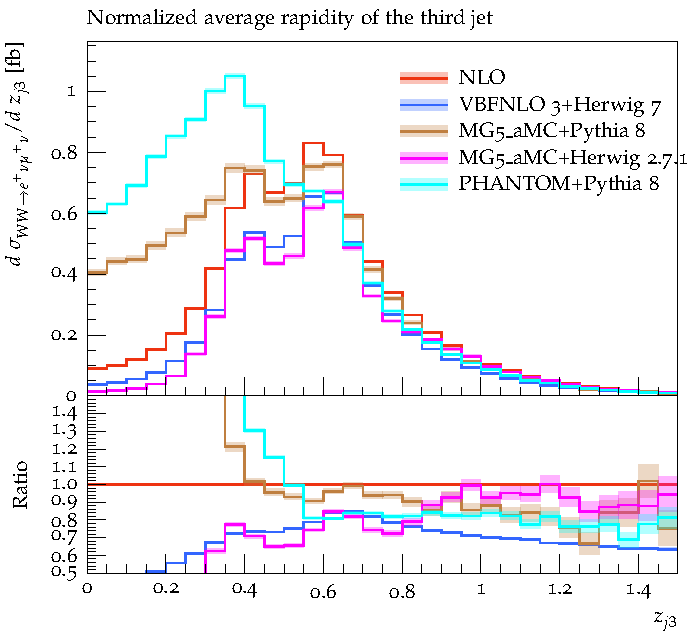
\includegraphics[width=0.47\textwidth]{figures/LOPS/z_j3.pdf}
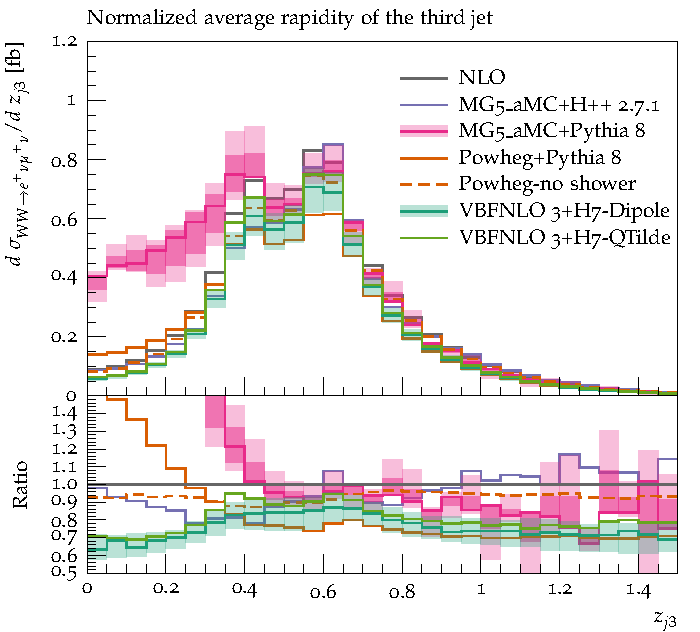
\includegraphics[width=0.47\textwidth]{figures/NLOPS/z_j3.pdf}
\caption{Differential distribution in the 
Zeppenfeld variable of the third-hardest jet
from predictions matched to parton shower, at LO (left) or NLO (right) accuracy (upper plot), compared with the fixed-NLO result computed with {\sc VBFNLO} (lower plot). At NLO+PS accuracy, for
    {\sc VBFNLO}+{\sc Herwig7-Dipole}, the three-point scale uncertainties are shown, while for {\sc MG5\_aMC}+{\sc Pythia8} the darker and lighter bands correspond  
    respectively to the nine-point scale uncertainty and the scale and PDF uncertainties combined linearly. 
    The predictions are obtained in the fiducial region described in Sec.~\ref{subsec:inputpar}.}
\label{fig:PSz3}
\end{figure*}
